\section{LLM Decontaminator}
\label{sec:llm-decontaminator}

% In this section, we propose a novel contamination detection method that can cost-effectively and accurately measure the degree of contamination of a dataset relative to a benchmark. 

In this section, we propose a new contamination detection method that accurately removes rephrased samples from a dataset relative to a benchmark.


\subsection{Algorithm}

% In the previous section, we discovered that embedding similarity search outperforms n-grams in terms of its capacity to identify rephrase contamination. 

% Why is embedding similarity search rarely used? First, there are a lot of false positives and false negatives, which makes it inaccurate. Second, establishing a threshold is necessary for embedding similarity search. It is impossible to establish a single threshold because it differs significantly for benchmarks used in different fields and subjects.


% The limited use of embedding similarity search can be attributed to its susceptibility to false positives/negatives and the challenge of setting a consistent threshold across diverse benchmarks.
% Embedding similarity search is rarely used because of the requirement to specify a threshold and its low precision.


% We suggest the "LLM decontaminator," a highly effective method, to overcome these two problems. There are two steps in this algorithm: First, for each test case in the benchmark, we use embedding similarity search to determine the top-k training data items with the highest similarity. According to the top-k training items, we create k potentially contaminated pairs for each test case. Then, we check each pair for contamination using a powerful LLM like GPT-4. With this method, we can precisely determine the benchmark's contamination status with only k times the amount of test case inquiries.

In Section~\ref{sec:background}, we discuss the limitations of existing detection methods including n-gram overlap and embedding similarity search.
To address the limitations, we introduce the ``LLM decontaminator'' in Algorithm \ref{algorith:detect-algo}. This method involves two steps: First, for each test case, it identifies the top-k training items with the highest similarity using the embedding similarity search. 
% From these items, it generates k potential rephrased pairs. \weilin{this sentence is repetitive} 
Each pair is evaluated whether they are the same by an advanced LLM, such as GPT-4.
This approach helps to determine how many rephrased samples there are in a dataset with a moderate computational overhead.
% This approach achieves precise rephrasing assessment with a computational overhead of k times the number of test cases. \weilin{this sentence is hard to understand}
``Template'' is a structured prompt that, when paired with a test case and training case, instructs the ``LLMDetector'' to carry out a comparison and return either `True' or `False'. 
In this context, `True' indicates that the training case might be a rephrased sample of the test case. ``LLMDetector'' is a high-quality LLM like GPT-4.
``TopKSimilarity'' identifies the top k most similar samples in the training data using embedding similarity search.

\begin{algorithm}
\caption{The algorithm for LLM decontaminator}
\label{algorith:detect-algo}

\begin{algorithmic}[1]
\ENSURE \( \text{Decontaminate}(TrainSet, TestSet, k, Template) \) 
\STATE \( Contamination \leftarrow \emptyset \)
\FOR{\(t\) in \(TestSet\)}
    %\STATE \(potentialContamination \leftarrow TopKSimilarity(TrainSet, t, k)\)
    \FOR{\(c\) in TopKSimilarity(\(TrainSet\), $t$, $k$)}
        \STATE \(s \leftarrow \text{LLMDetector}(Template, t, c)\)
        \IF{\(s = True\)}
            \STATE \( Contamination \leftarrow Contamination\cup\{(t, c)\} \)
        \ENDIF
    \ENDFOR
\ENDFOR
\RETURN \( Contamination \)
\end{algorithmic}
\end{algorithm}
\belowcaptionskip=10pt
% {\footnotesize
% Note: Template is a prompt template that, when used with a test case and training case, enables the Model to make a comparison and prompts the Model to only return `True' or `False'. `True' here denotes that the test case has been contaminated by the train case. Prompts in the TrainSet that are top-k similar to the test case embedding can be excluded using the TopKSimilarity filter. Parse can translate 'True' or 'False' string values into 'True' or 'False' boolean values.
% Note: ``Template'' is a structured prompt that, when paired with a test case and training case, instructs the ``LLMDetector'' to carry out a comparison and return either `True' or `False'. 
% In this context, `True' indicates that the training case might be a rephrased sample of the test case. ``LLMDetector'' is a high-quality LLM like GPT-4.
% ``TopKSimilarity'' identifies the top k most similar samples in the training data using embedding similarity search.
% \todo{what's topk similarity?}

% }

% \todo{Complexity and Cost?}


\subsection{Contamination Detection Visualization}

% To better illustrate the role of the LLM decontaminator, we introduce the memorization-generalization spectrum. Each point on this spectrum represents the similarity of a (train case, test case) pair. Points closer to the left end of the spectrum signify that the pair is closer to memorization, while those near the right end indicate a tendency toward generalization.
% The block labeled (train set, test set) represents the collection of (train case, test case) pairs where each test case in the test set is paired with its closest match in the train set.
% The discernment boundary of the detecting method is shown by the red dashed line. The detection method is highly likely to flag points to the left of this line as contaminated.

% \todo{1. embedding similarity position is confusing 2. train/test set? how to interpret}

% To illustrate the role of the LLM decontaminator, Figure \ref{fig:spectrum} displays a Venn diagram of contamination and different detection methods. 
In Figure \ref{fig:spectrum} we present a Venn diagram of contamination and different detection methods.
The LLM decontaminator takes advantage of embedding similarity search, which helps it rapidly filter out possible possible contamination.
In addition, it utilizes the strong LLMs' reliable judgments.
We show that n-gram overlap detection can result in a higher false negative rate when detecting rephrased samples, and embedding similarity search detects many false positives with a high threshold. Notably, the LLM decontaminator showcases higher accuracy while detecting rephrased samples.
% \todo{add some high-level insight}
% Solid sections indicate training data and its subsets, while hollow sections highlight areas marked as contaminated by detection methods.
% Notably, the LLM decontaminator showcases higher accuracy.
% Embedding similarity search detects broadly but with many false positives. N-gram overlap has a limited ability to spot rephrased samples. The LLM decontaminator refines the results from embedding similarity search using LLMs, providing a precise and efficient contamination assessment.
See Section \ref{sec:rephrase-exp} for comprehensive experimental results.

\begin{figure*}[h]
\centering
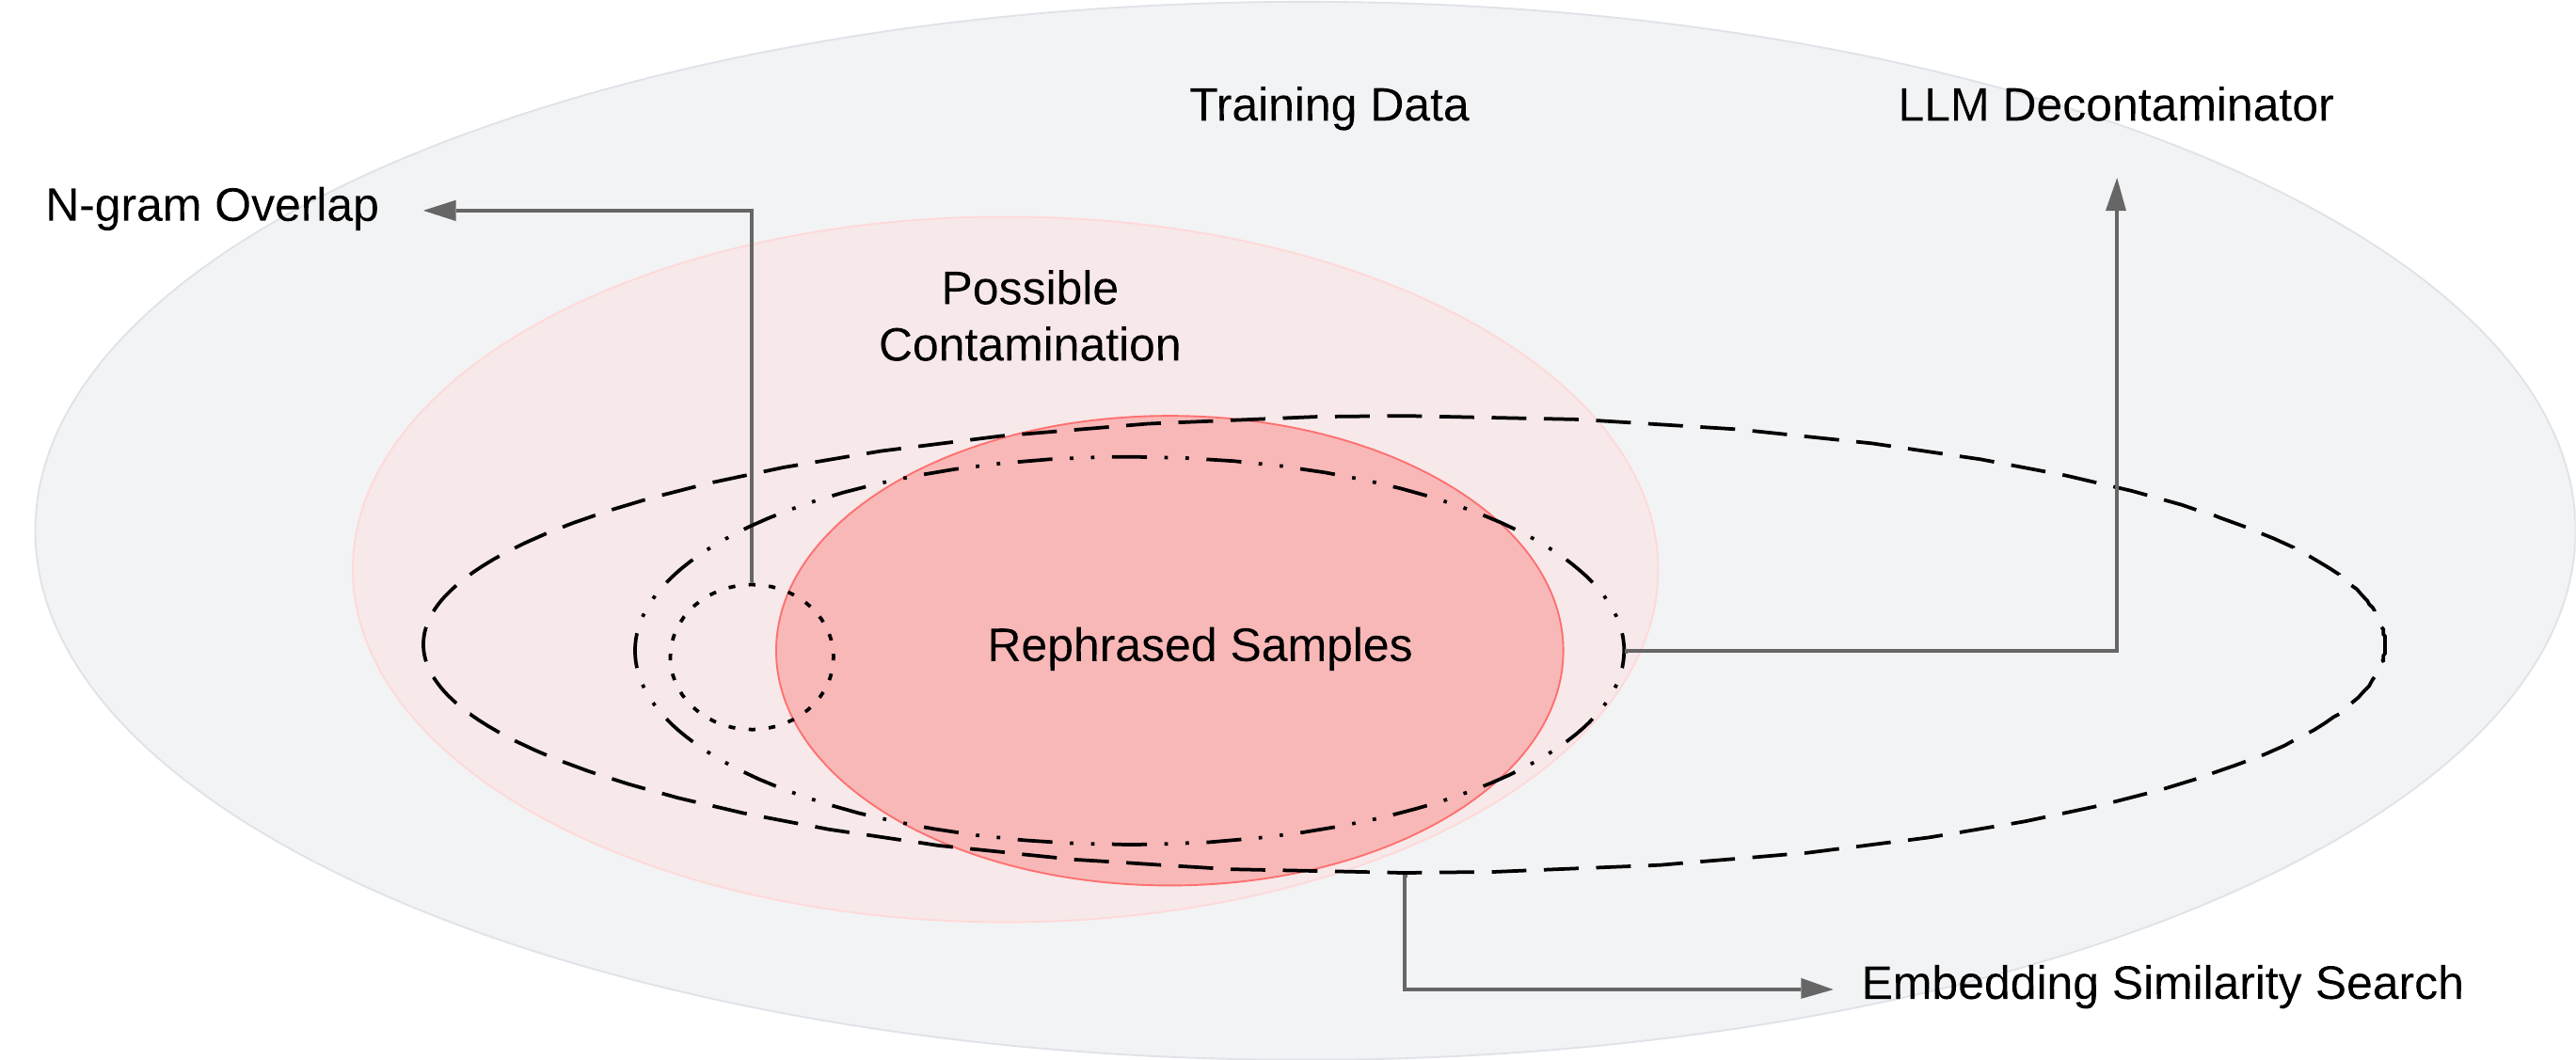
\includegraphics[width=0.9\textwidth]{contamination_venn-v2.png}
\caption{Venn graph depicting training data subsets and contamination detection ranges.
% Solid sections indicate training data and its subsets, while hollow sections highlight areas marked as contaminated by detection methods.
The solid circle represents the training data and its subsets.
The dashed circles enclose areas flagged for potential contamination by detection methods within the dataset.
Notably, the LLM decontaminator showcases higher accuracy.
Embedding similarity search detects broadly but with many false positives. N-gram overlap has a limited ability to spot rephrased samples. The LLM decontaminator refines the results from embedding similarity search using LLMs, providing a precise and efficient contamination assessment.
}
\label{fig:spectrum}
\vspace{-25pt}
\end{figure*}


% \subsection{experiments}

% The rephrase contamination dataset created in section 3.4 was examined using the LLM Decontaminator. The complete f1 score table can be found in the appendix.




% \subsection{real world dataset}

% % We applied the decontamination method on popular real-world datasets and discovered a substantial amount of rephrase contamination. It's highly likely that these contaminations, similar to the experiments in section 3.4, inflate the benchmark evaluation. We will present the number of detected rephrase contaminations as well as some rephrased test cases.

% We used the LLM Decontamination on well-known real-world datasets and discovered significant rephrase contamination. Similar to the tests in section 3.4, it is very likely that these contaminations exaggerate the benchmark evaluation. 


% \textbf{FLAN}~\citep{longpre2023flan} is a sizable knowledge training dataset. We chose to examine a subset called CoT, which accounts for 1.63\% of FLAN, due to its size and variety of data sources. We utilized GPT-4 for detection and set k=1 for the decontamination parameters. The findings show that 76 test cases, or 0.543\% of the MMLU test set, were contaminated.


% \begin{tcolorbox}[title={FLAN CoT Contamination Example}]
% \begin{multicols}{2}

% \textbf{MMLU test} \newline 

% Question: \\
% What type of meat is on a traditional Reuben sandwich?
%     \begin{itemize}
%         \item[A.] turkey
%         \item[B.] bologna
%         \item[C.] corned beef
%         \item[D.] pepperoni
%     \end{itemize}

% Answer: C

% \columnbreak 

% \textbf{FLAN CoT} \newline

% Question: \\
% The Reuben sandwich is an American hot sandwich composed of corned beef, Swiss cheese, sauerkraut, and Russian dressing, grilled between slices of rye bread. Several variants exist.

% What is the meat in a reuben sandwich? Let's have some stream of consciousness first. \\
% % Answer: \\
% % The relevant sentence in the passage is: The Reuben sandwich is an American hot sandwich composed of corned beef, Swiss cheese, sauerkraut, and Russian dressing, grilled between slices of rye bread. So, the answer is corned beef.
% \end{multicols}
% \end{tcolorbox}


% \textbf{CodeAlpaca}~\citep{codealpaca} contains 20K instruction-following data used for fine-tuning the Code Alpaca model. 
% Codealpaca-20K was used to train a number of well-known models, including Tulu~\citep{wang2023far}. 
% We also employed GPT-4 for detection with k=1 as the parameter. The results reveal that there are 21 contaminated test cases on HumanEval, accounting for 12.8\% of HumanEval.


% \begin{tcolorbox}[title={CodeAlpaca Contamination Example}]
% \begin{multicols}{2}

% % HumanEval test code
% \begin{tcolorbox}[title={HumanEval test}, enhanced, colback=white, boxrule=1pt, sharp corners, boxsep=5pt, left=5pt, right=5pt, top=5pt, bottom=5pt]
% \fontsize{8pt}{9.6pt}\selectfont
% \begin{minted}{python}
% def sum_to_n(n: int):
%     """sum_to_n is a function that 
%     sums numbers from 1 to n.
%     >>> sum_to_n(30)
%     465
%     >>> sum_to_n(100)
%     5050
%     >>> sum_to_n(5)
%     15
%     >>> sum_to_n(10)
%     55
%     >>> sum_to_n(1)
%     1
%     """
%     return sum(range(n + 1))
% \end{minted}
% \end{tcolorbox}

% \columnbreak

% % CodeAlpaca code
% \begin{tcolorbox}[title={CodeAlpaca}, enhanced, colback=white, boxrule=1pt, sharp corners, boxsep=5pt, left=5pt, right=5pt, top=5pt, bottom=5pt]
% \fontsize{8pt}{9.6pt}\selectfont
% \begin{minted}{python}
% """
% Create a code that summation 
% of all numbers between 1 to n.
% """

% def sum_all_nums(n):
%     res = 0
    
%     for i in range(1, n+1):
%         res += i
    
%     return res


% print(sum_all_nums(n)) # 15
% \end{minted}
% \end{tcolorbox}

% \end{multicols}
% \end{tcolorbox}




% \textbf{MATH}~\citep{hendrycksmath2021} is one of the most widely used datasets for training mathematical capabilities. It encompasses various branches of mathematics, including algebra, geometry, number theory, and more. It has been utilized in the construction of many math datasets, including MathInstruct~\citep{yue2023mammoth}. Within MATH, we identified 79 instances of self-rephrase contamination, making up 1.58\% of the MATH test set.


% \begin{tcolorbox}[title={MATH Contamination Example}]
% \begin{multicols}{2}

% \textbf{MATH test} \newline 

% How many three-digit positive integers are multiples of 11?

% \columnbreak 

% \textbf{MATH} \newline

% How many positive 3-digit numbers are divisible by 11?

% \end{multicols}
% \end{tcolorbox}

% We examined numerous datasets in addition to those already stated. The appendix contains information on the possible contamination of these datasets as well as examples of contamination.

